\documentclass{article}
\usepackage[margin=1in]{geometry}  % set the margins to 1in on all sides
\usepackage{graphicx}              % to include figures
\usepackage{epstopdf}
\usepackage{amsmath}               % great math stuff
\usepackage{amsfonts}              % for blackboard bold, etc
\usepackage{amsthm}                % better theorem environments
\usepackage{amssymb}
\usepackage[english]{babel}
\usepackage[utf8]{inputenc}
\usepackage{fancyhdr}
\usepackage{tikz}
\usepackage{lipsum,array,amsmath}
\usetikzlibrary{positioning,automata}
\usetikzlibrary{arrows.meta}
\usepackage{pgfplots}
\usepackage{amsmath}
\DeclareMathOperator*{\argmax}{argmax}
\DeclareMathOperator*{\argmin}{argmin}
\usepackage{hyperref}
\usepackage{caption}
\usepackage{subcaption}
\usepackage{float}
\usepackage{algorithm,algorithmic}
\usepackage{bbold}
\usepackage{tabularx}
\usepackage{mathtools}

\pagestyle{fancy}
\fancyhf{}
\rhead{Islam A. Ali}
\lhead{CMPUT-566: Project Report}
\rfoot{Page \thepage}
\lfoot{\scriptsize{}}


\begin{document}


% =================== Header ====================
\begin{center}
{\bf CMPUT 566: Introduction to Machine Learning}  \\
{Car Evaluation Classification: Project Report} \\
\vspace{.1in}
{\em Islam A. Ali}\\
{\em Student ID: 1633813}\\
{\em iaali@ualberta.ca}\\
\end{center}
\noindent\rule{\textwidth}{1pt}
% ==========================================================================

\section*{Abstract}
Data classification is considered a very important corner stone in supervised learning and in machine learning in general. That's due to the wide spectrum of problems in which intelligent classification is needed, and also the available algorithms that proven proper performance when tested. In this report, we explore different ML classification algorithms in order to evaluate acceptability of cars using a publicly available car evaluation data set. The algorithms tested include: Naive Bayes, KNN, Decision Trees, Random Forest, and SVM. The implementation was done using Python3, numpy, pandas, and skLearn libraries. Finally, The algorithms are compared to each other based on the accuracy as the main measure of success.

\noindent\rule{\textwidth}{1pt}
% ==========================================================================

\section{Problem Formulation}
The problem at hand is classification problem with labeled data set with an objective to correctly determine the level of acceptability of car based on a number of provided features. The following subsections show more information about the data set, validation mechanism, and also the performance metrics measured when executing classification with different algorithms.

\subsection{Selected Dataset}
\textbf{Car Evaluation Data Set} \footnote{The data set is available at: https://archive.ics.uci.edu/ml/datasets/Car+Evaluation} was utilized in this project to train ML models and to test their performances. The data set consists of 1728 labeled samples with six different categorical features, as well as a categorical label. The following table illustrates of the available features, its semantic meaning and their values range.

\begin{table}[H]
\centering
\caption{Car Evaluation Data set Details}
\begin{tabular}{l|c|l|c}
\hline
\multicolumn{1}{c|}{\textbf{Data Set Field}} & \textbf{Type} & \multicolumn{1}{c|}{\textbf{Definition}} & \textbf{Range}           \\ \hline
buying                                       & Feature       & Buying price                             & $\lbrace$ v-high, high, med, low $\rbrace$   \\
maint                                        & Feature       & Maintenance price                        & $\lbrace$ v-high, high, med, low $\rbrace$   \\
doors                                        & Feature       & Number of doors                          & $\lbrace$ 2, 3, 4, 5-more $\rbrace$          \\
persons                                      & Feature       & Capacity in terms of persons to carry    & $\lbrace$ 2, 4, more $\rbrace$               \\
lug\_boot                                    & Feature       & The size of the luggage boot             & $\lbrace$ small, med, big  $\rbrace$         \\
safety                                       & Feature       & Estimated safety of the car              & $\lbrace$ low, med, high $\rbrace$          \\ \hline
car\_class                                   & Label         & Car acceptability                        & $\lbrace$ unacc, acc, good, v-good $\rbrace$ \\ \hline
\end{tabular}
\end{table}

\subsection{Training-Validation-Testing Framework}
The training-validation-testing framework is adopted in this work in order to have a concrete and realistic measure of algorithm's success. For that, k-fold with a choice of 5 folds approach was utilized due to the size of the data set which does not exceed \~ 1800 samples. Other approaches such as leave-out validation may not be suitable for small data sets and more applicable with larger and more generic data sets. 

\subsection{Measure of Success}
The main measure of success is the classification accuracy given by: 
\begin{equation}
Accuracy = \frac{\sum_{m=1}^{M} \mathbb{1} \lbrace \hat{t} = t \rbrace }{M}
\end{equation}
Other performance metrics are also reported and used in the comparison such that, precision, recall, F1-score, and confusion matrix. 
% ==========================================================================

\section{Data Set Representation}
The categorical values provided in the original data set is not suitable for usage with different machine learning algorithms inside the sklearn library. For this reason, this categorical values require transformation into numerical data to become compatible with the library's algorithms. Two different representations of features are applicable: the first one is what we call decimal representation, and the second one is binary representation. In the following subsections, both representation are illustrated. Moreover, both representations were tested and the corresponding performance was reported with an aim to provide an analysis of the impact of features representation on the classification accuracy. 

\subsection{Decimal Features Representation}
The first representation is converting each data feature field into a set of decimal values corresponding to the categorical values, which means that the resulting feature vector will have the same size as the data set attributes size which is $1 \times 6$ for each data sample.

\begin{table}[H]
\centering
\caption{Decimal Features Mapping}
\begin{tabular}{l|c|c}
\hline
\multicolumn{1}{c|}{\textbf{Data Set Field}} & \textbf{Numerical Range} & \multicolumn{1}{l}{\textbf{Categorical Range}} \\ \hline
buying                                       & $\lbrace$ v-high, high, med, low $\rbrace$    & $\lbrace$ 5, 4, 3, 1 $\rbrace$                                     \\
maint                                        & $\lbrace$ v-high, high, med, low $\rbrace$    & $\lbrace$ 5, 4, 3, 1 $\rbrace$                                    \\
doors                                        & $\lbrace$ 2, 3, 4, 5-more $\rbrace$            & $\lbrace$ 2, 3, 4, 5 $\rbrace$                                     \\
persons                                      & $\lbrace$ 2, 4, more $\rbrace$                & $\lbrace$ 2, 4, 5 $\rbrace$                                       \\
lug\_boot                                    & $\lbrace$ small, med, big $\rbrace$           & $\lbrace$ 1, 3, 5 $\rbrace$                                        \\
safety                                       & $\lbrace$ low, med, high $\rbrace$             & $\lbrace$ 1, 3, 5 $\rbrace$                                        \\ \hline
\end{tabular}
\end{table}

\subsection{Binary Features Representation}
The second representation is representing features by values indicators which increases the size of the input features vector. This service is provided by the $get_dummies$ function available in the $pandas$ package in Python3. The size of the input feature vector will become $1 \times 21$ for each data sample. The increase in the size of the feature vector is beneficial for some classification algorithms such as the naive bayes classification.

\subsection{Label Representation}
The car label must be a single value for each data sample, which follows the definition of the decimal feature representation. The following is the mapping used for the output label from the categorical space to the numerical space. The following table shows how mapping is done for the car acceptability output labels. 

\begin{table}[H]
\centering
\caption{Decimal Labels Mapping}
\begin{tabular}{l|c|l}
\hline
\multicolumn{1}{c|}{\textbf{Data Set Field}} & \textbf{Categorical Range} & \textbf{Categorical Range}     \\ \hline
car\_class                                   & $\lbrace$ unacc, acc, good, v-good $\rbrace$  & \multicolumn{1}{c}{ $\lbrace$ 1, 2, 3, 4 $\rbrace$ } \\ \hline
\end{tabular}
\end{table}

% ==========================================================================

\section{Classification Baseline}
The classification base line is defined to classifying all samples as being the dominating class. The following graph provide the frequency of each car label.

\begin{figure}[H]
\centering
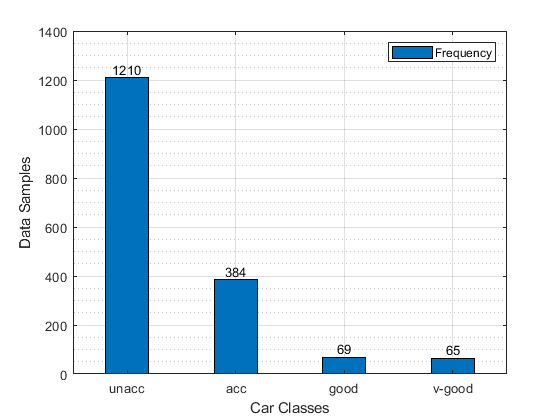
\includegraphics[width=0.7\textwidth]{../Figures/baseline_bar.png}
\caption{Frequency of different car classes in the data set}
\end{figure}

The graph shows that the dominating class is "unacc" with a frequency of $70.023 \% $, meaning that classifying all samples to belong to "unacc" class will result in an accuracy of $70.023 \% $, which is considered the base line accuracy that should be enhanced or surpassed by the usage of ML classification algorithms. It also shows that the data is highly skewed towards the "unacc" class, which makes it more challenging to have a generalized model with high accuracy. It also adds another motivation for the usage of k-fold validation to ensure generalization.
% ==========================================================================

\section{Experimented Classification Algorithms}

\subsection{Naive Bayes}
Naive Bayes is a simple probabilistic classifier, that depends on applying Bayes theorem with a naive features' independence assumption. This assumption may not hold in a wide range of cases as this kind of correlation may exist and may have a strong impact on the quality of classification. The classifier also makes benefit from the extended number of features and may have a performance improvement with larger feature vector size.
\subsubsection*{Hyper-parameters}
\begin{table}[H]
\centering
\begin{tabularx}{0.8\textwidth}{l|X|X}
\hline
\textbf{Hyperparameter} & \multicolumn{1}{c|}{\textbf{Definition}}    & \multicolumn{1}{c}{\textbf{Tuning Technique}}   \\ \hline
alpha                   & Additive smoothing to categorical data & Exhaustive search from 0 to 1 with 0.1 step size \\ \hline
\end{tabularx}
\end{table}

\subsection{K-Nearest Neighbors (KNN)}
KNN is a classification algorithm that depends on assign the class value of a certain data sample to be the result of a majority vote of it K-nearest neighbors. The value of K is determined by the training phase and picked to maximize the validation accuracy. In case of having k=1, the classification is determined based on the single nearest sample to the unknown sample. 
\subsubsection*{Hyper-parameters}
\begin{table}[H]
\centering
\begin{tabularx}{0.8\textwidth}{l|X|X}
\hline
\textbf{Hyperparameter} & \multicolumn{1}{c|}{\textbf{Definition}}      & \multicolumn{1}{c}{\textbf{Tuning Technique}}  \\ \hline
n\_neighbors            & Number of neighbors to use for classification & Exhaustive search from 1 to 30 with 1 step size \\ \hline
\end{tabularx}
\end{table}


\subsection{Decision Tree}
The decision tree is a classification algorithms that depends on having a tree-like structure where nodes represent a certain feature and its outward edges represent decisions made based on the feature value. The leaf nodes (which has no outward edges) on the other hand, represent the outcome of the decision tree after passing through multiple checks on the way. The training procedure tries to find out the optimal structure for this tree, the split locations, and features choices that can maximize the validation accuracy. 
\subsubsection*{Hyper-parameters}
\begin{table}[H]
\centering
\begin{tabularx}{0.8\textwidth}{l|X|X}
\hline
\textbf{Hyperparameter} & \multicolumn{1}{c|}{\textbf{Definition}}              & \multicolumn{1}{c}{\textbf{Tuning Technique}}                   \\ \hline
criterion               & The function used to measure the quality of the split & Random search in the range \{'gini', 'entropy'\}                 \\ \hline
max\_depth              & The maximum depth of the tree                         & Random search in the range \{None, 1, 5, 10, 30, 50, 100, 1000\} \\ \hline
min\_samples\_split     & The minimum number of samples needed to split a node  & Random search in the range from 2 to 10 with an step = 1         \\ \hline
min\_samples\_leaf      & The minimum samples required to form a leaf node      & Random search in the range from 1 to 10 with a step = 1          \\ \hline
\end{tabularx}
\end{table}

\subsection{Random Forest}
Random forest is another classification algorithm that depends heavily on the definition we made for the decision tree. That's due to the fact that it is an ensemble classifier that has multiple decision trees running at the same time, and the output should be the majority vote for these estimators. The parameters are very similar to that of the decision tree with few extra ones to control the forest structure. A good point to mention here, is that in order to fairly evaluate the random forest performance against the decision tree, one shall use the same set of common parameters in both to ensure that the only difference is the forest structure not the trees themselves. 
\subsubsection*{Hyper-parameters}
\begin{table}[H]
\centering
\begin{tabularx}{0.8\textwidth}{l|X|X}
\hline
\textbf{Hyperparameter} & \multicolumn{1}{c|}{\textbf{Definition}}              & \multicolumn{1}{c}{\textbf{Tuning Technique}}                             \\ \hline
criterion               & The function used to measure the quality of the split & Random search in the range \{'gini', 'entropy'\}                           \\ \hline
max\_depth              & The maximum depth of the tree                         & Random search in the range \{None, 1, 5, 10, 30, 50, 100, 300, 500, 1000\} \\ \hline
n\_estimators           & The number of trees to present in the forest          & Random search in the range \{10, 30, 50, 100, 500, 1000\}                  \\ \hline
max\_features           & The number of features to consider when splitting     & Random search in the range \{'auto', 'sqrt', 'log2', None\}                \\ \hline
min\_samples\_split     & The minimum number of samples needed to split a node  & Random search in the range from 2 to 10 with an step = 1                   \\ \hline
min\_samples\_leaf      & The minimum samples required to form a leaf node      & Random search in the range from 1 to 10 with a step = 1                    \\ \hline
\end{tabularx}
\end{table}

\subsection{Support Vector Machines (SVM)}
SVM is a classification algorithm that aims at finding the best hyperplane to separate two classes with the maximum margin between the classes available in the data set. In case of having more than two classes, SVM uses the strategy of one-vs-all in order to classify the correct class. Hyperplane is mainly the decision boundary between classes while the data points located at either sides of the decision boundary is called the support vectors due to the fact that the algorithm depends on these samples to decide on the best hyperplane. 
\subsubsection*{Hyper-parameters}
\begin{table}[H]
\centering
\begin{tabularx}{0.8\textwidth}{l|X|X}
\hline
\textbf{Hyperparameter} & \multicolumn{1}{c|}{\textbf{Definition}}        & \multicolumn{1}{c}{\textbf{Tuning Technique}}                                                                                 \\ \hline
C                       & Regularization parameter, strictly positive     & Random search in the range \{0.001, 0.003, 0.005, 0.01, 0.03, 0.05, 0.1, 0.3, 0.5, 1, 3, 5, 10, 30, 50, 100\}                  \\ \hline
kernel                  & The kernel to be used with SVM                  & Random search in the range \{'linear', 'poly', 'rbf', 'sigmoid'\}                                                              \\ \hline
degree                  & Polynomial degree for 'poly' kernel             & Random search in the range from 1 to 10 with a step = 1                                                                        \\ \hline
gamma                   & Kernel coefficient for 'poly', 'rbf', 'sigmoid' & Random search in the range \{'scale', 'auto', 0.001, 0.003, 0.005, 0.01, 0.03, 0.05, 0.1, 0.3, 0.5, 1, 3, 5, 10, 30, 50, 100\} \\ \hline
\end{tabularx}
\end{table}

% ==========================================================================
\newpage
\section{Results and Discussion}
In this section, the experimental results of the 5 algorithms are provided with discussion of the findings. The results include reporting of the accuracy, precision, recall, F1-measure, and the confusion matrix. 

\subsection{Accuracy}

\begin{figure}[H]
\centering
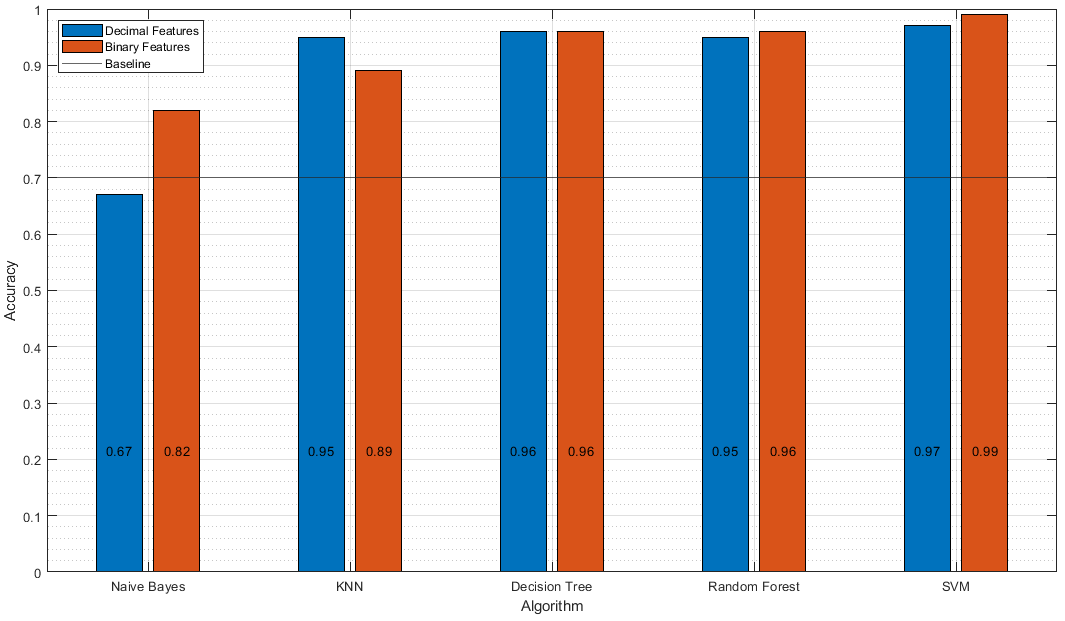
\includegraphics[width=\textwidth]{../Figures/accuracy.png}
\caption{Classification Accuracy in case of Decimal and Binary Features}
\end{figure}

\subsection{Precision}

\begin{figure}[H]
\centering
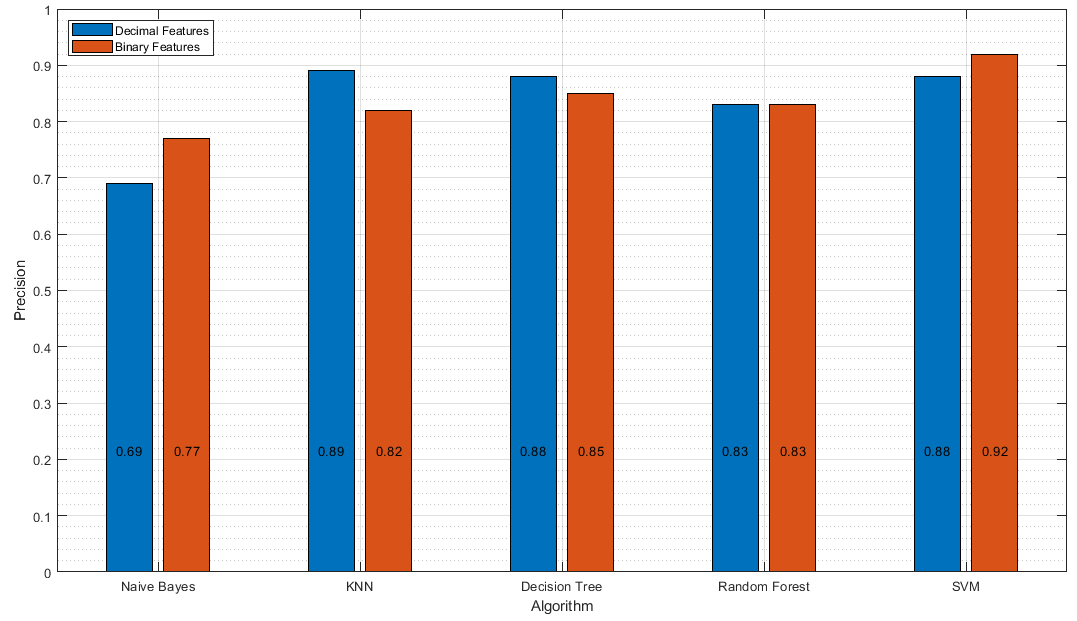
\includegraphics[width=\textwidth]{../Figures/precision.png}
\caption{Classification Accuracy in case of Decimal and Binary Features}
\end{figure}

\subsection{Recall}

\begin{figure}[H]
\centering
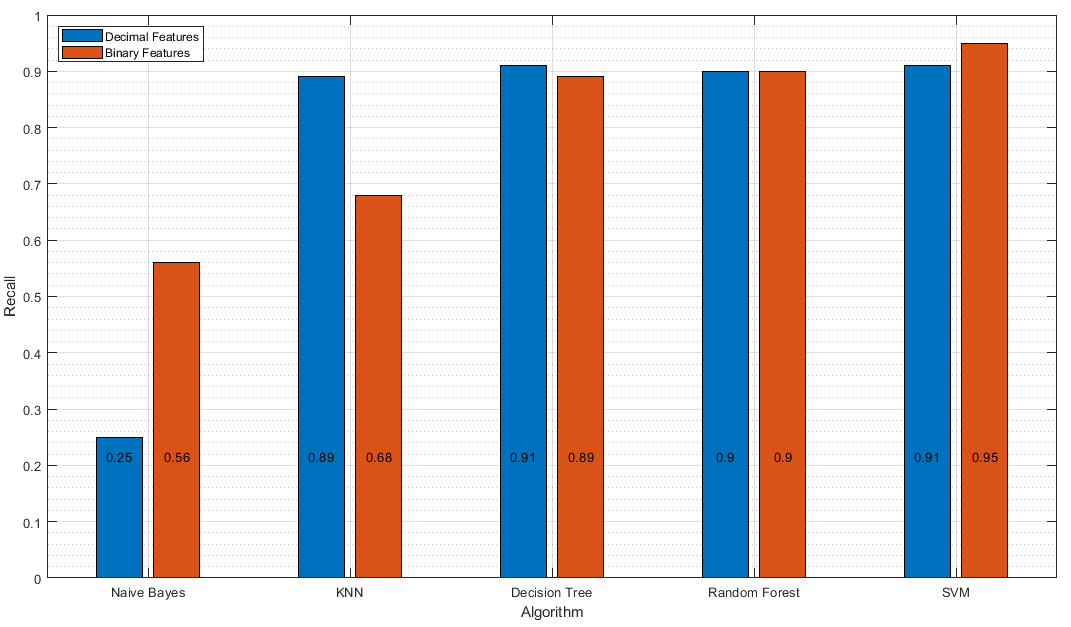
\includegraphics[width=\textwidth]{../Figures/recall.png}
\caption{Classification Accuracy in case of Decimal and Binary Features}
\end{figure}

\subsection{F1-Measure}

\begin{figure}[H]
\centering
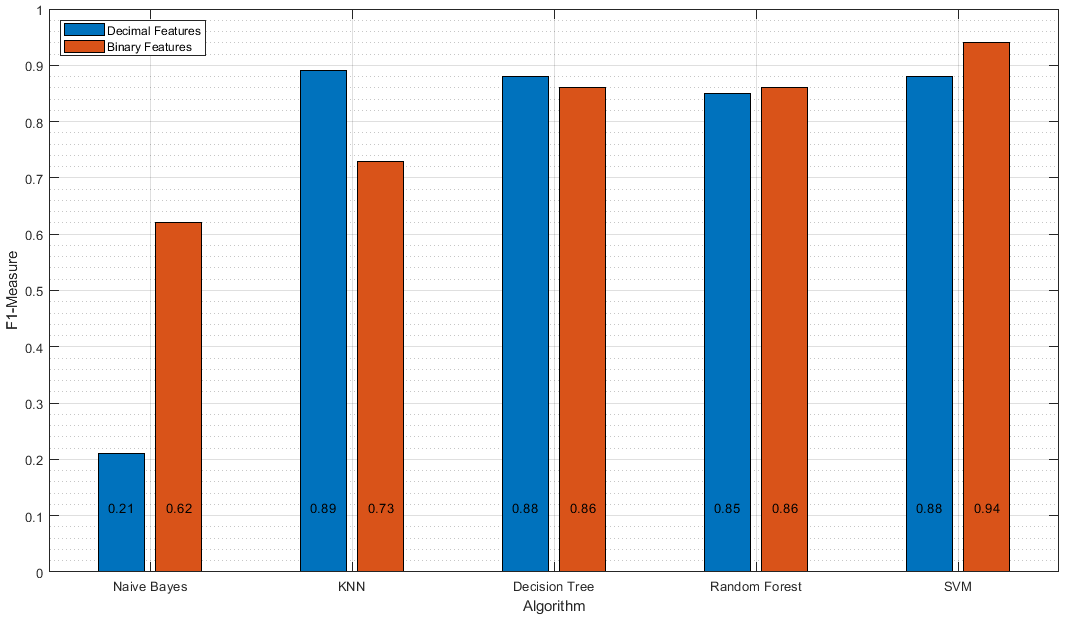
\includegraphics[width=\textwidth]{../Figures/f1.png}
\caption{Classification Accuracy in case of Decimal and Binary Features}
\end{figure}

\subsection{Confusion Matrix}

\begin{figure}[H]
     \centering
     \hspace*{\fill}
     \begin{subfigure}[b]{0.35\textwidth}
         \centering
         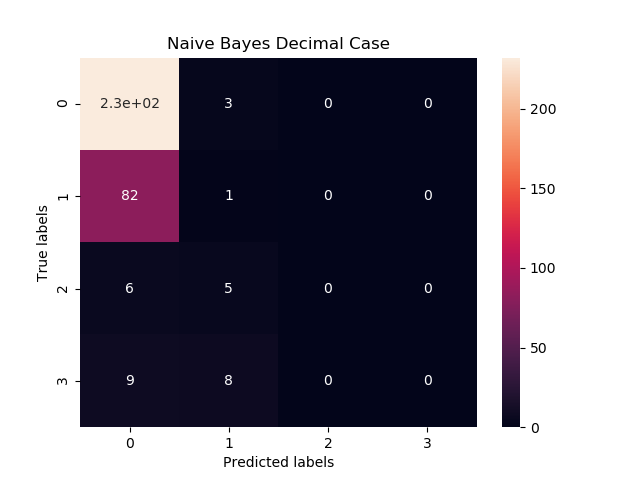
\includegraphics[width=\textwidth]{../Figures/Naive Bayes Decimal Case_conf_mat.png}
         \caption{Decimal Features}
     \end{subfigure}
     \hfill
     \begin{subfigure}[b]{0.35\textwidth}
         \centering
         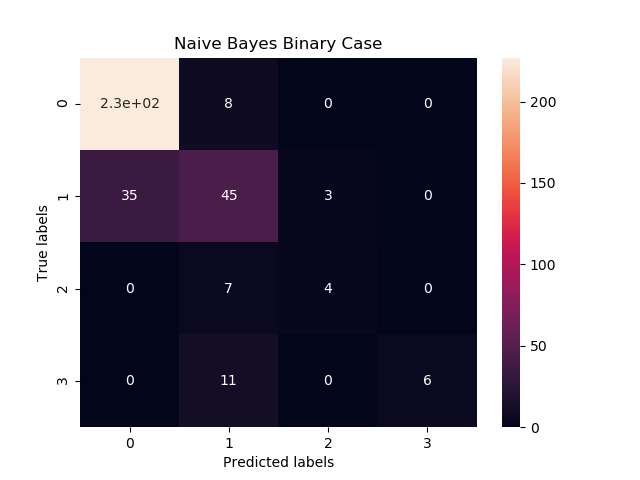
\includegraphics[width=\textwidth]{../Figures/Naive Bayes Binary Case_conf_mat.png}
         \caption{Binary Features}
     \end{subfigure}
     \hspace*{\fill}
     \caption{Naive Bayes Confusion Matrix}
\end{figure}

\begin{figure}[H]
     \centering
     \hspace*{\fill}
     \begin{subfigure}[b]{0.35\textwidth}
         \centering
         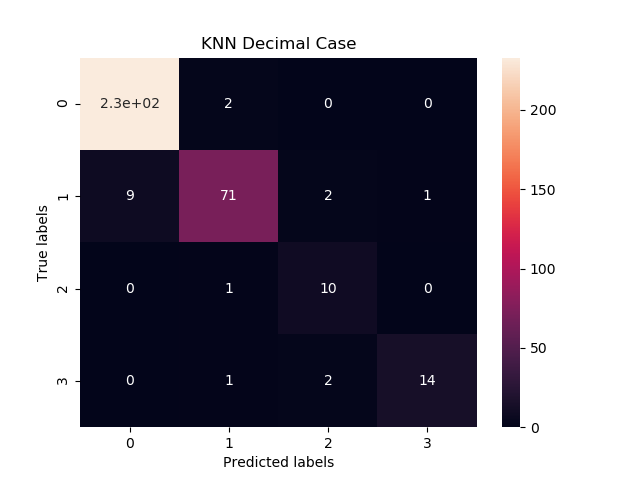
\includegraphics[width=\textwidth]{../Figures/KNN Decimal Case_conf_mat.png}
         \caption{Decimal Features}
     \end{subfigure}
     \hfill
     \begin{subfigure}[b]{0.35\textwidth}
         \centering
         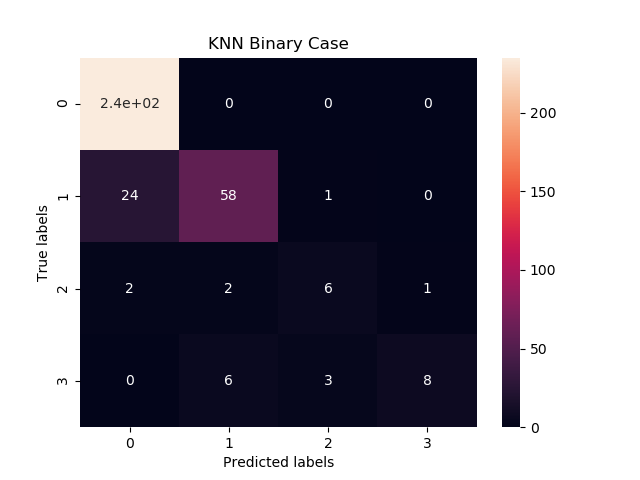
\includegraphics[width=\textwidth]{../Figures/KNN Binary Case_conf_mat.png}
         \caption{Binary Features}
     \end{subfigure}
     \hspace*{\fill}
     \caption{KNN Confusion Matrix}
\end{figure}

\begin{figure}[H]
     \centering
     \hspace*{\fill}
     \begin{subfigure}[b]{0.35\textwidth}
         \centering
         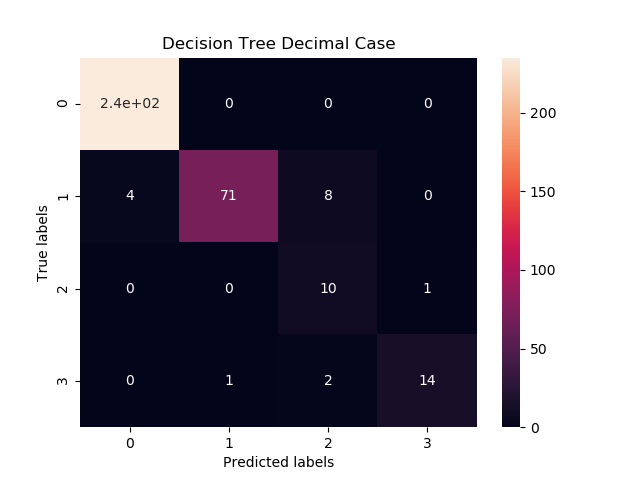
\includegraphics[width=\textwidth]{../Figures/Decision Tree Decimal Case_conf_mat.png}
         \caption{Decimal Features}
     \end{subfigure}
     \hfill
     \begin{subfigure}[b]{0.35\textwidth}
         \centering
         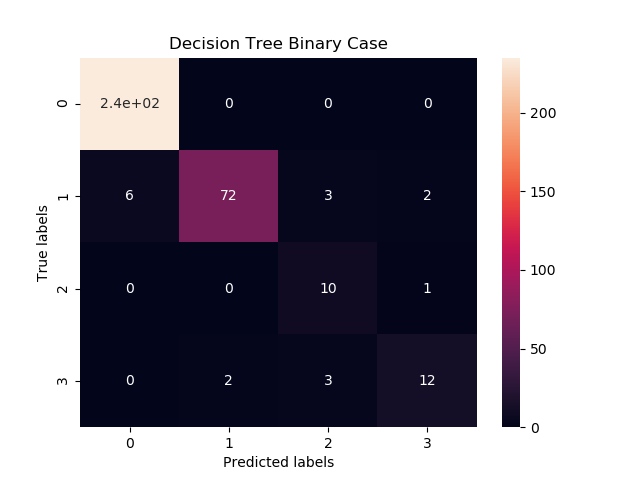
\includegraphics[width=\textwidth]{../Figures/Decision Tree Binary Case_conf_mat.png}
         \caption{Binary Features}
     \end{subfigure}
     \hspace*{\fill}
     \caption{Decision Tree Confusion Matrix}
\end{figure}

\begin{figure}[H]
     \centering
     \hspace*{\fill}
     \begin{subfigure}[b]{0.35\textwidth}
         \centering
         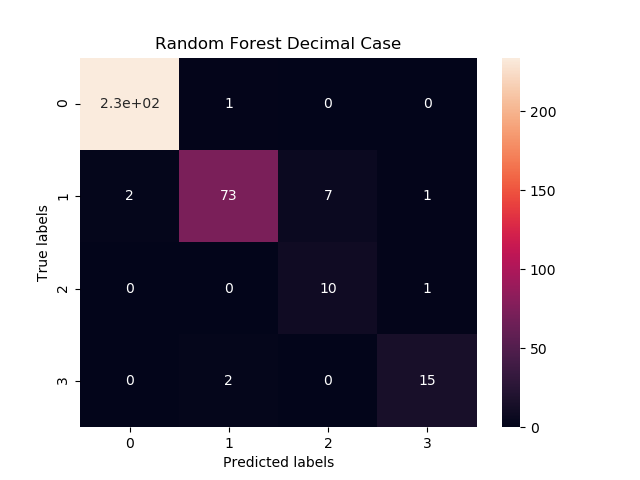
\includegraphics[width=\textwidth]{../Figures/Random Forest Decimal Case_conf_mat.png}
         \caption{Decimal Features}
     \end{subfigure}
     \hfill
     \begin{subfigure}[b]{0.35\textwidth}
         \centering
         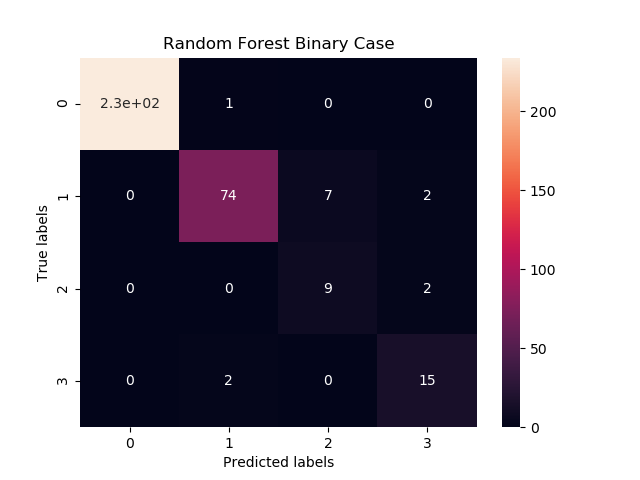
\includegraphics[width=\textwidth]{../Figures/Random Forest Binary Case_conf_mat.png}
         \caption{Binary Features}
     \end{subfigure}
     \hspace*{\fill}
     \caption{Random Forest Confusion Matrix}
\end{figure}

\begin{figure}[H]
     \centering
     \hspace*{\fill}
     \begin{subfigure}[b]{0.35\textwidth}
         \centering
         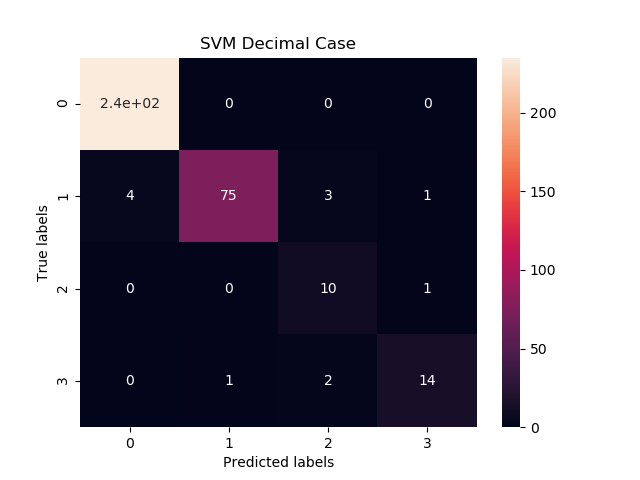
\includegraphics[width=\textwidth]{../Figures/SVM Decimal Case_conf_mat.png}
         \caption{Decimal Features}
     \end{subfigure}
     \hfill
     \begin{subfigure}[b]{0.35\textwidth}
         \centering
         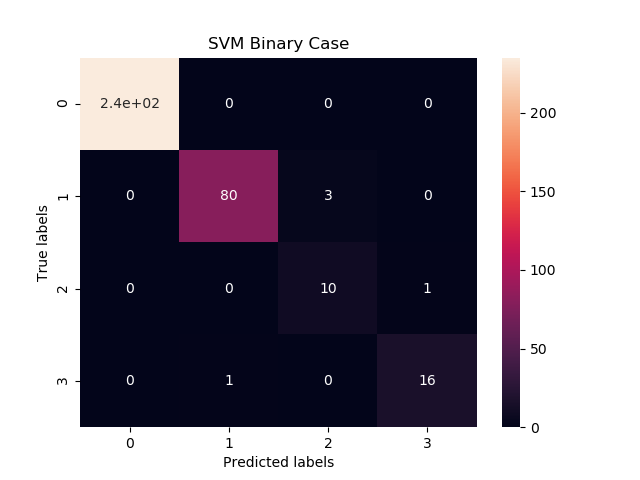
\includegraphics[width=\textwidth]{../Figures/SVM Binary Case_conf_mat.png}
         \caption{Binary Features}
     \end{subfigure}
     \hspace*{\fill}
     \caption{SVM Confusion Matrix}
\end{figure}

% ==========================================================================

\section{Conclusion}


% ==========================================================================
\end{document}